
\documentclass{article}
\usepackage[]{graphicx}

\begin{document}

\title{All Figures}

\maketitle

\newpage

\section{Raw data}
\newpage

\begin{figure}
  \centering
  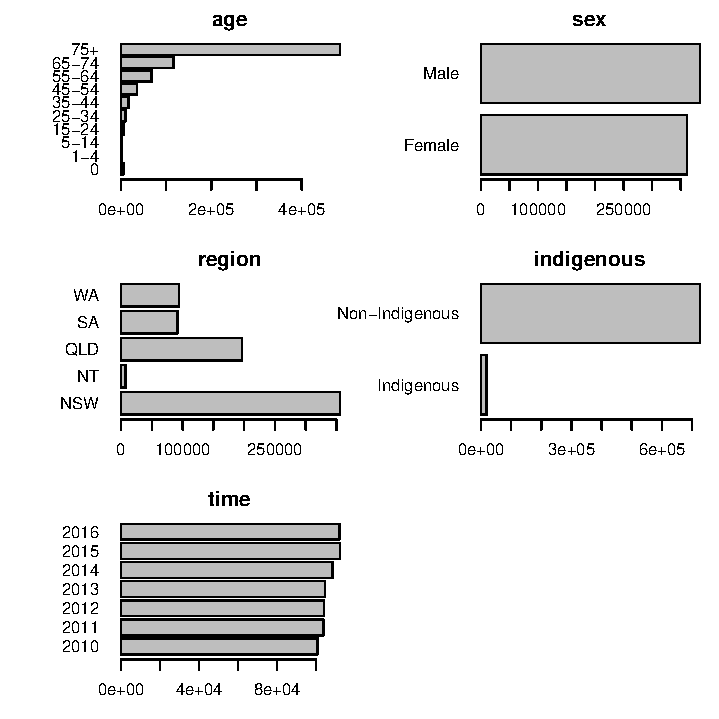
\includegraphics{out/fig_data_deaths}
\end{figure}
\newpage

\begin{figure}
  \centering
  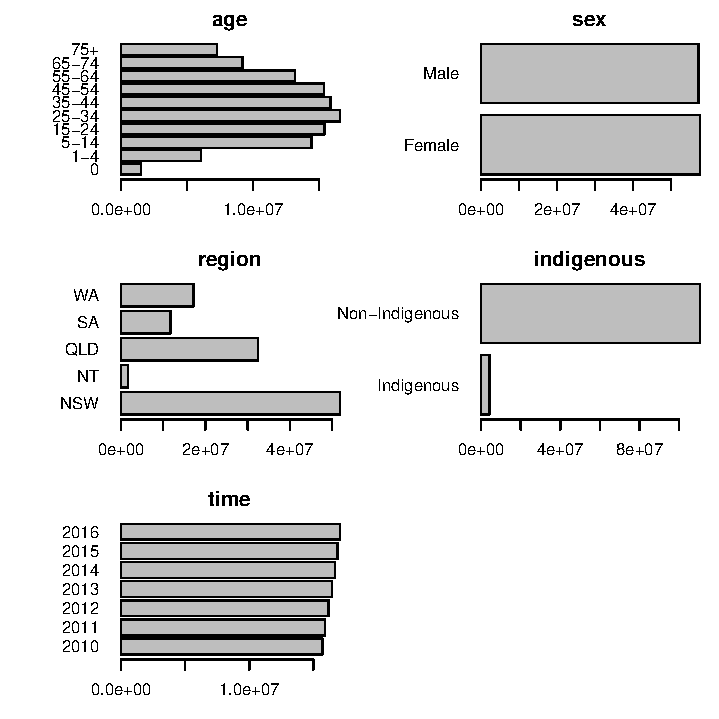
\includegraphics{out/fig_data_population}
\end{figure}
\newpage

\clearpage
\section{Direct estimates of rates}
\newpage

\begin{figure}
  \centering
  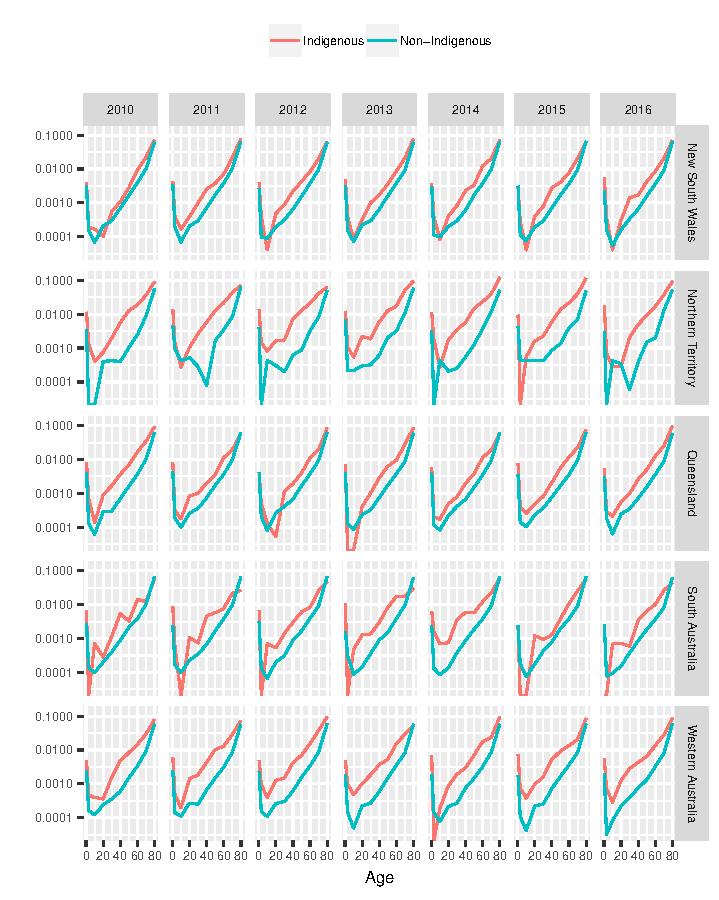
\includegraphics{out/fig_rates_direct_Female}
\end{figure}
\newpage

\begin{figure}
  \centering
  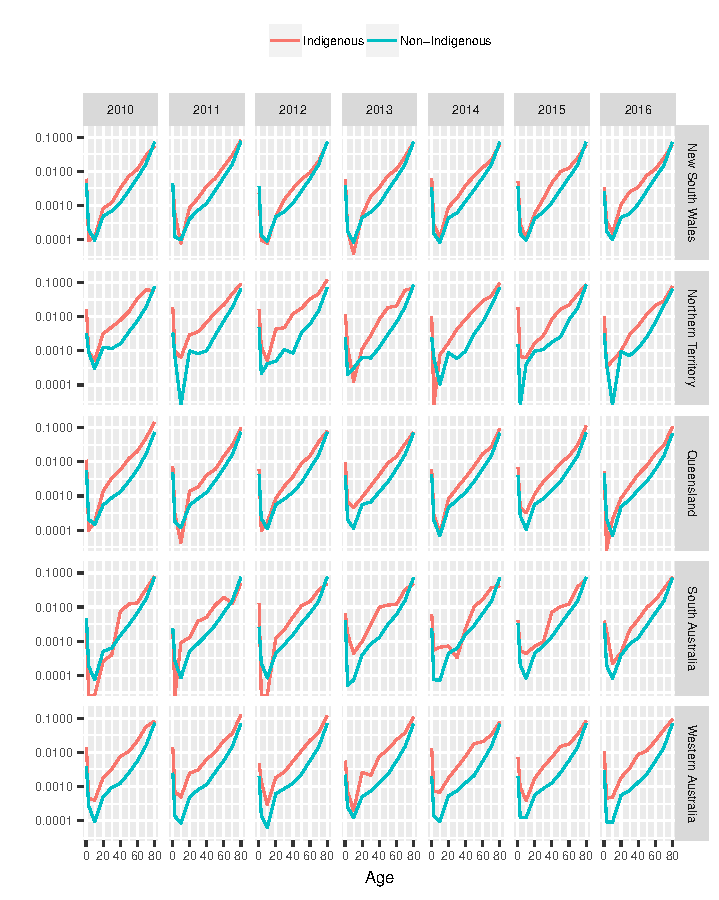
\includegraphics{out/fig_rates_direct_Male}
\end{figure}
\newpage

\clearpage
\section{Modelled estimates of rates}
\newpage

\begin{figure}
  \centering
  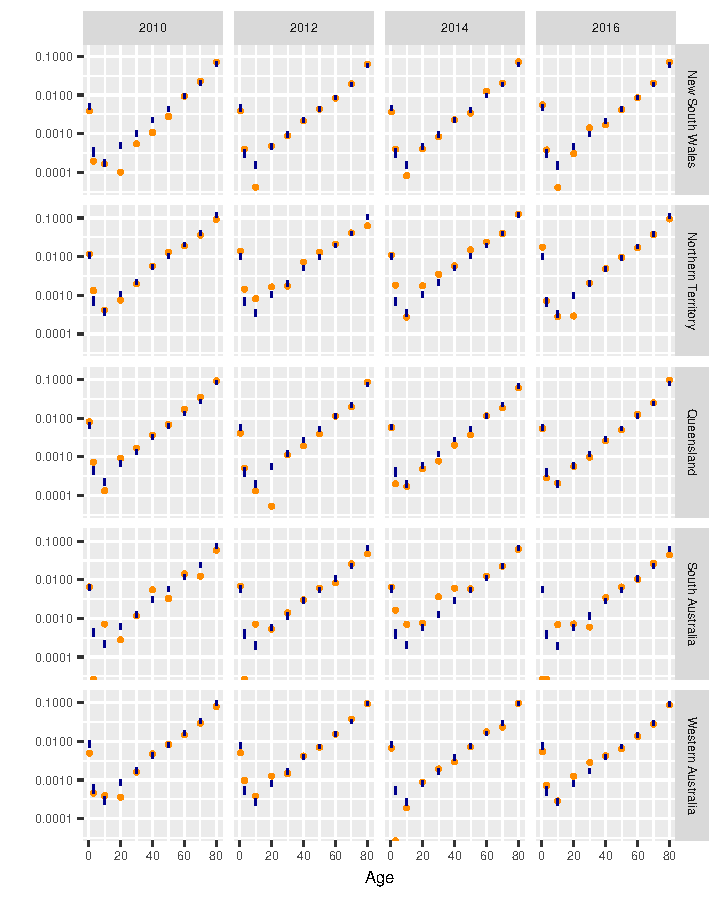
\includegraphics{out/fig_rates_modelled_Female_Indigenous_Baseline}
\end{figure}
\newpage

\begin{figure}
  \centering
  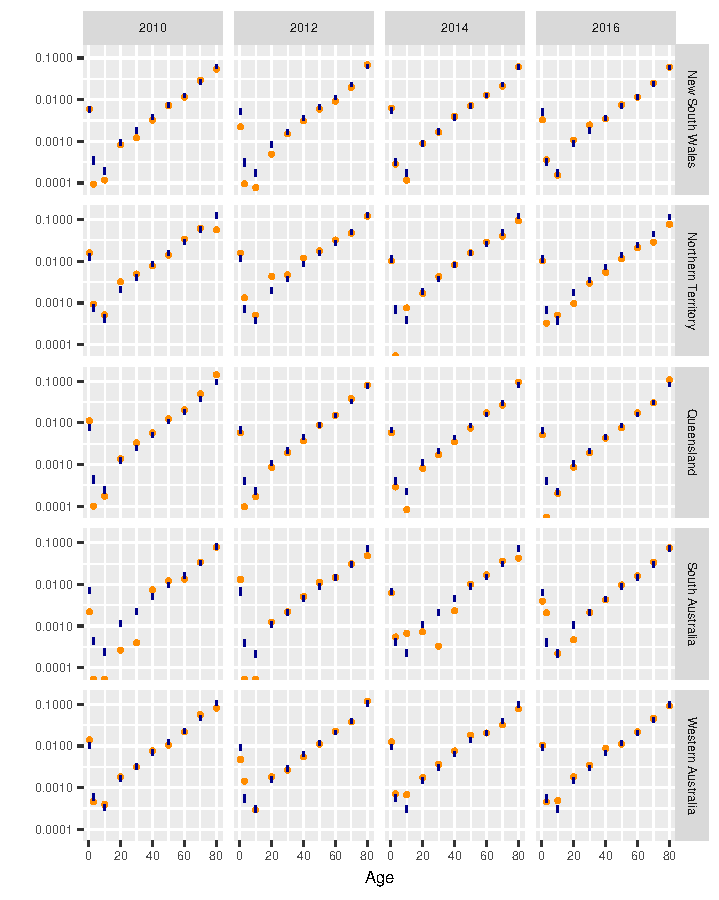
\includegraphics{out/fig_rates_modelled_Male_Indigenous_Baseline}
\end{figure}
\newpage

\begin{figure}
  \centering
  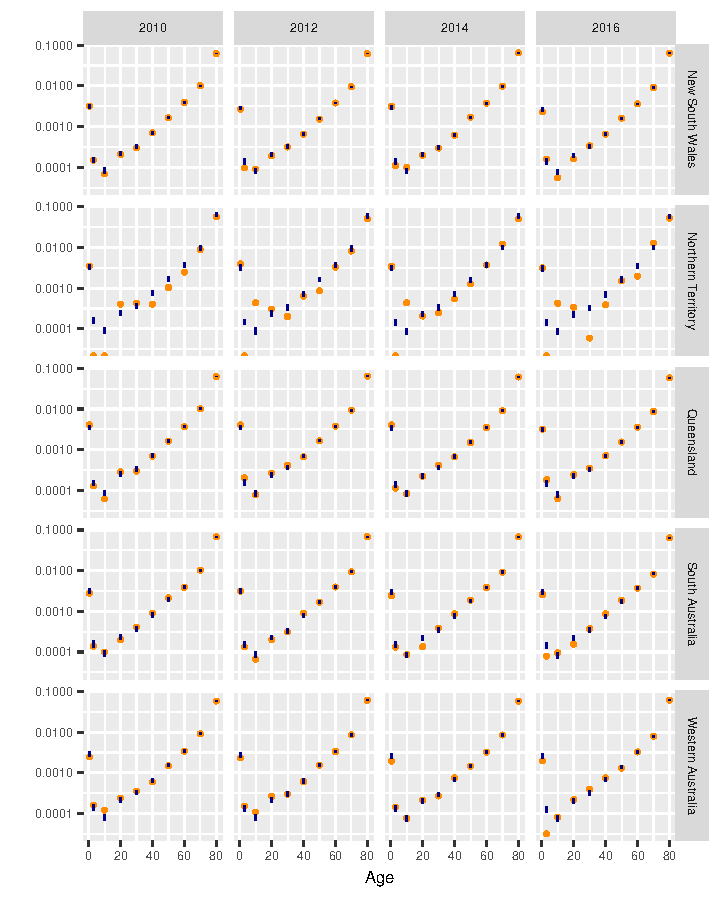
\includegraphics{out/fig_rates_modelled_Female_Non-Indigenous_Baseline}
\end{figure}
\newpage

\begin{figure}
  \centering
  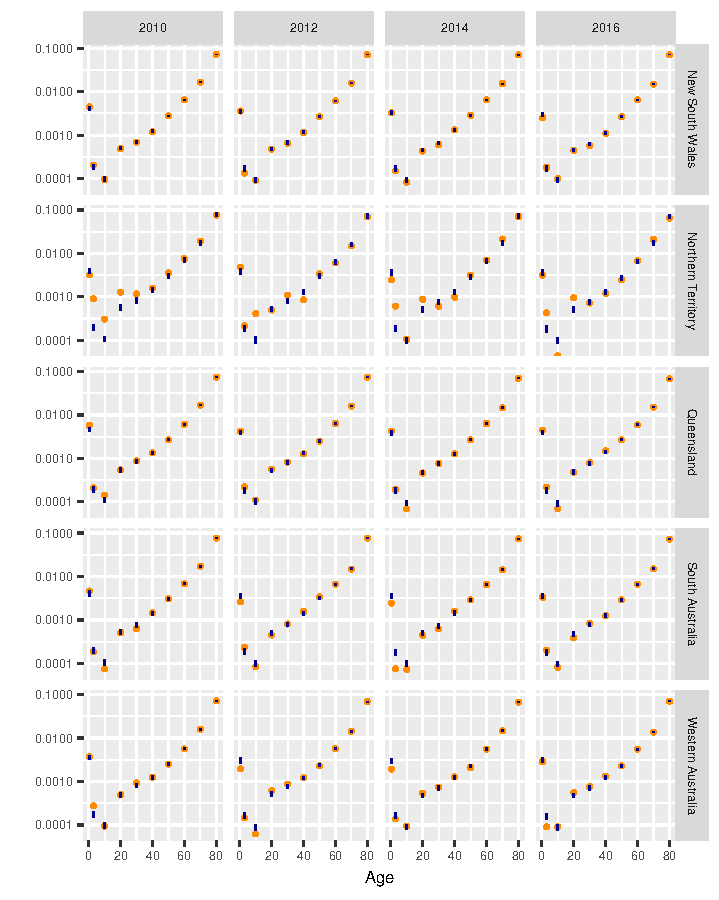
\includegraphics{out/fig_rates_modelled_Male_Non-Indigenous_Baseline}
\end{figure}
\newpage

\clearpage
\section{Replicate data}
\newpage

\begin{figure}
  \centering
  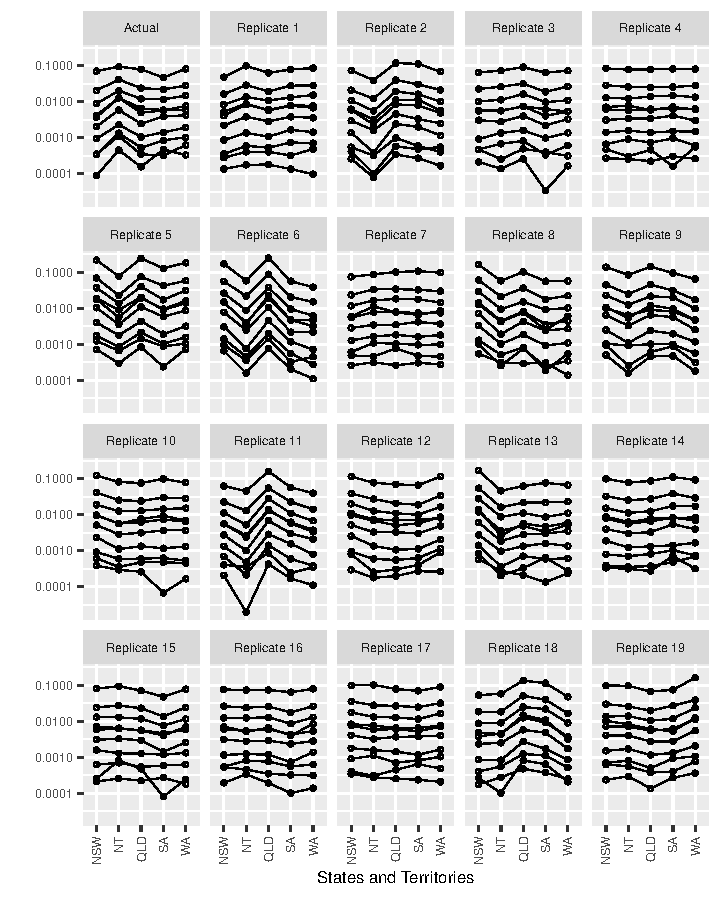
\includegraphics{out/fig_replicate_data_Female_Indigenous_Baseline}
\end{figure}
\newpage

\begin{figure}
  \centering
  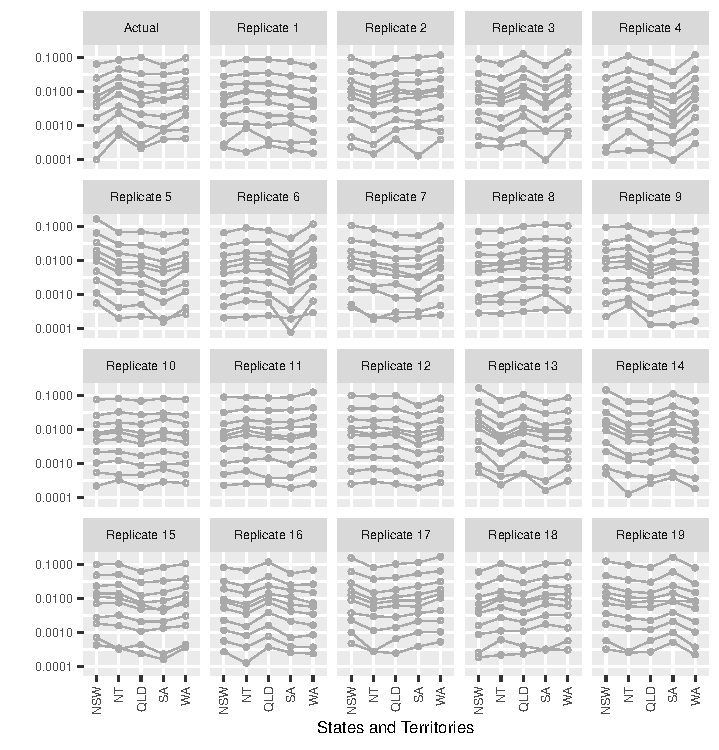
\includegraphics{out/fig_replicate_data_Male_Indigenous_Baseline}
\end{figure}
\newpage

\begin{figure}
  \centering
  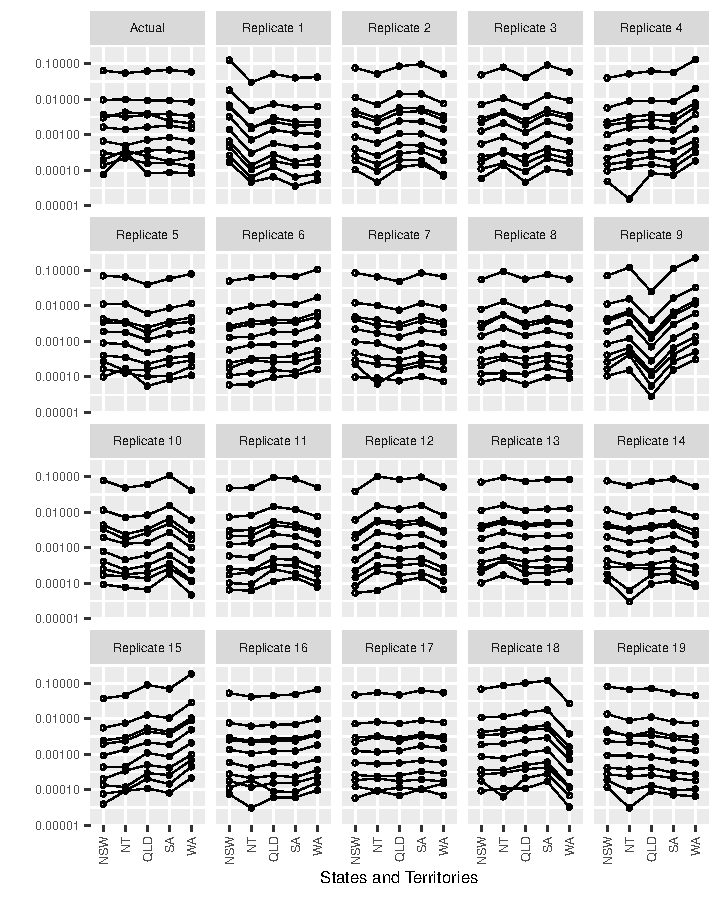
\includegraphics{out/fig_replicate_data_Female_Non-Indigenous_Baseline}
\end{figure}
\newpage

\begin{figure}
  \centering
  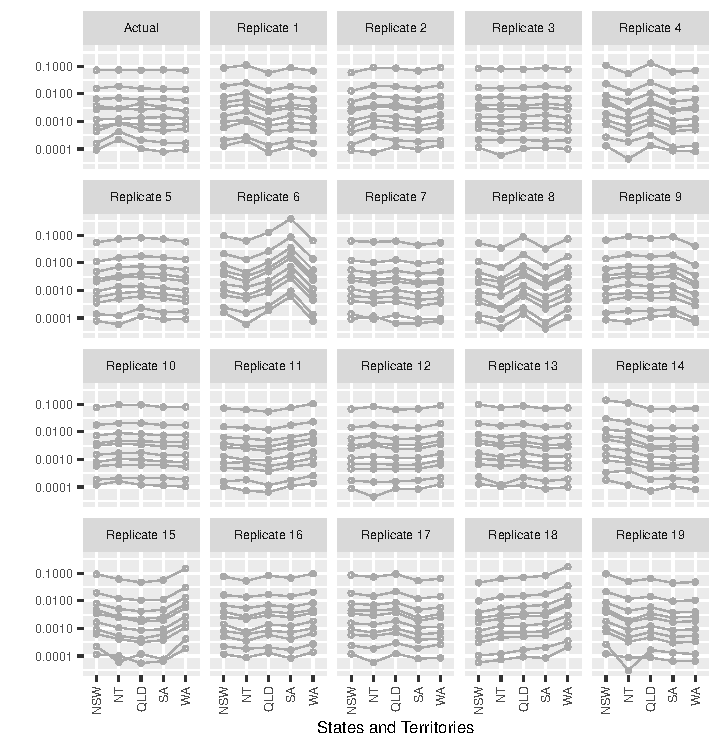
\includegraphics{out/fig_replicate_data_Male_Non-Indigenous_Baseline}
\end{figure}
\newpage


\clearpage
\section{Life expectancy}
\newpage

\begin{figure}
  \centering
  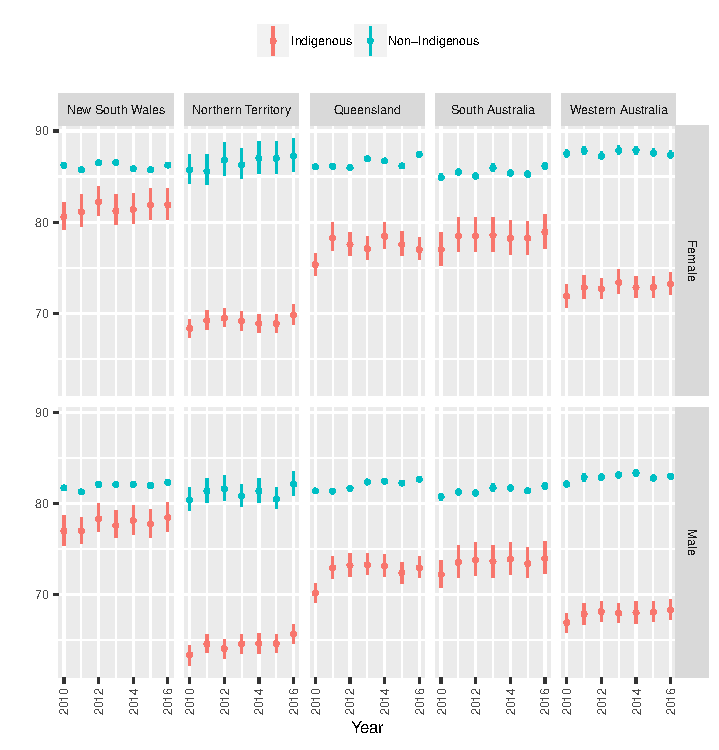
\includegraphics{out/fig_life_expectancy_Baseline}
\end{figure}
\newpage




\end{document}
